\documentclass[11pt]{article}
\usepackage[a4paper,margin=0.9in]{geometry}
\usepackage[T1]{fontenc}
\usepackage{lmodern}
\usepackage{amsmath,amssymb,booktabs,graphicx,microtype,xcolor}
\usepackage[round,numbers,sort&compress]{natbib}
\usepackage[colorlinks=true,linkcolor=teal,citecolor=teal,urlcolor=teal]{hyperref}
\newcommand{\project}{NeuroStreamLab}
\newcommand{\SoftwareVersion}{0.1.0}
\newcommand{\TotalSubjects}{8}
\newcommand{\TrainTrials}{582}
\newcommand{\TestTrials}{507}
\newcommand{\EpochSeconds}{3.0}
\newcommand{\SeedValue}{42}
\newcommand{\MaxEpochs}{30}
\newcommand{\BootstrapSamples}{2000}
\newcommand{\LatencyCalls}{100}
\newcommand{\PhysioCSPClean}{55.9}
\newcommand{\PhysioCSPLatency}{0.010}
\newcommand{\PhysioCSPNoise}{50.0}
\newcommand{\PhysioCSPDropout}{50.0}
\newcommand{\PhysioCSPAmplitude}{49.1}
\newcommand{\PhysioCSPAdapted}{51.8}
\newcommand{\PhysioEEGNetClean}{44.6}
\newcommand{\PhysioEEGNetLatency}{0.157}
\newcommand{\PhysioEEGNetNoise}{50.0}
\newcommand{\PhysioEEGNetDropout}{50.0}
\newcommand{\PhysioEEGNetAmplitude}{50.4}
\newcommand{\PhysioEEGNetAdapted}{45.9}
\newcommand{\PhysioBandpowerClean}{60.9}
\newcommand{\PhysioBandpowerLatency}{0.010}
\newcommand{\PhysioBandpowerNoise}{48.8}
\newcommand{\PhysioBandpowerDropout}{50.0}
\newcommand{\PhysioBandpowerAmplitude}{50.5}
\newcommand{\PhysioBandpowerAdapted}{51.1}
\newcommand{\BNCICSPClean}{73.1}
\newcommand{\BNCICSPLatency}{0.011}
\newcommand{\BNCICSPNoise}{50.0}
\newcommand{\BNCICSPDropout}{50.0}
\newcommand{\BNCICSPAmplitude}{62.3}
\newcommand{\BNCICSPAdapted}{73.1}
\newcommand{\BNCIEEGNetClean}{50.0}
\newcommand{\BNCIEEGNetLatency}{0.179}
\newcommand{\BNCIEEGNetNoise}{50.9}
\newcommand{\BNCIEEGNetDropout}{51.2}
\newcommand{\BNCIEEGNetAmplitude}{50.5}
\newcommand{\BNCIEEGNetAdapted}{51.2}
\newcommand{\BNCIBandpowerClean}{67.1}
\newcommand{\BNCIBandpowerLatency}{0.009}
\newcommand{\BNCIBandpowerNoise}{54.6}
\newcommand{\BNCIBandpowerDropout}{50.0}
\newcommand{\BNCIBandpowerAmplitude}{63.9}
\newcommand{\BNCIBandpowerAdapted}{68.8}

\newcommand{\SyntheticPipelineMedian}{0.794}
\newcommand{\SyntheticPipelinePninetyfive}{1.352}
\newcommand{\SyntheticFrames}{120}
\newcommand{\SyntheticPredictions}{0}
\newcommand{\SyntheticGaps}{4}
\newcommand{\ReplayPipelineMedian}{0.102}
\newcommand{\ReplayPipelinePninetyfive}{0.229}
\newcommand{\ReplayFrames}{500}
\newcommand{\ReplayPredictions}{16}
\newcommand{\ReplayGaps}{0}


\title{NeuroStreamLab: Hardware-Free Real-Time BCI Development and EEG Replay Robustness}
\author{Syed Abdullah Imam\\University of North Texas}
\date{}
\begin{document}
\maketitle
\begin{abstract}
Developing brain computer interface software requires acquisition, signal processing, decoding, timing, and application integration before a useful experiment can be run. Access to EEG hardware can constrain this engineering work, while offline classification alone does not exercise a streaming application. We present \project{}, an open source local environment that separates acquisition from timestamped processing and supports BrainFlow synthetic streams, recorded EEG replay, and an explicit future hardware adapter. A browser console exposes signals, probabilities, temporal decisions, perturbations, and runtime telemetry. We evaluate log bandpower logistic regression, common spatial patterns with linear discriminant analysis, and a CPU-trained EEGNet on held-out imagined left versus right hand trials from PhysioNet and on cross-session BNCI motor imagery. The exploratory cohort contains \TotalSubjects{} participants and \TestTrials{} test trials. Controlled noise, channel loss, amplitude scaling, drift, and mixed shifts are applied before trial-local filtering. Clean mean balanced accuracy for CSP plus LDA is \PhysioCSPClean{}\% on PhysioNet and \BNCICSPClean{}\% on BNCI. Under the largest tested additive noise, these means are \PhysioCSPNoise{}\% and \BNCICSPNoise{}\%. An unlabeled, causal RMS-alignment reference strategy gives condition-dependent recovery rather than a universal improvement. Measured inference and software-processing timings are stored separately from accuracy. All numerical tables and figures are generated from machine-readable artifacts. The results demonstrate a reproducible development workflow, not clinical utility or physical acquisition validation. The small cohort, limited electrode set, and offline trial preprocessing constrain generalization.
\end{abstract}

\section{Introduction}
An EEG-based brain computer interface combines several software responsibilities. A source must supply correctly ordered channels with timestamps. Preprocessing must respect acquisition timing. A decoder must provide probabilities whose temporal interpretation is explicit. An application must remain responsive when signals stop, channels fail, or predictions become uncertain. These responsibilities can be developed using recorded human EEG and synthetic engineering streams before buying an acquisition device.

The scientific question considered here is how motor imagery decoders respond to controlled signal degradation and distribution shift, and how a hardware-free environment can make those observations reproducible. A related question is whether a conservative unlabeled normalization strategy recovers performance under the chosen shifts. We use a small fixed cohort to exercise the complete software and publication workflow. We do not propose a new decoding algorithm or claim general model superiority.

The contribution is a source-independent local system with deterministic replay, explicit perturbation configurations, interchangeable decoders, a browser control application, and a traceable experiment-to-manuscript pipeline. Recorded replay preserves labeled trial boundaries and supplies held-out data incrementally. Synthetic acquisition tests engineering behavior but is never interpreted as motor imagery. No physical EEG hardware was used in this evaluation.

\section{Related work}
BCI2000 established a modular general-purpose environment linking acquisition, processing, and feedback \citep{schalk2004}. BrainFlow exposes compatible acquisition interfaces and dummy boards for software testing \citep{brainflow}. \project{} builds on these ecosystem ideas rather than replacing their hardware infrastructure. Its focus is local replay, configurable failure scenarios, and linked research artifacts.

MNE-Python supplies EEG readers, event extraction, and established signal-processing components \citep{mne}. MOABB standardizes dataset access and highlights the dependence of decoder comparisons on datasets and evaluation procedures \citep{moabb}. We use MNE to retrieve only the PhysioNet hand-imagery runs required by the binary protocol and MOABB for the multi-session BNCI adapter. Braindecode provides reusable neural architectures and training-oriented interfaces \citep{braindecode}. The neural baseline is its EEGNet implementation, based on the compact temporal and spatial convolution architecture described by \citet{eegnet}.

Common spatial patterns extract variance differences between classes and provide an established motor imagery reference \citep{csp}. Nonstationarity also motivates adaptation strategies that use unlabeled information \citep{adaptation}. Our expanding channel-RMS alignment is a simpler reference normalization strategy. It does not reproduce the classifier adaptation method in that work, and its inclusion is not a novelty claim.

\section{System design}
\begin{figure}[t]
\centering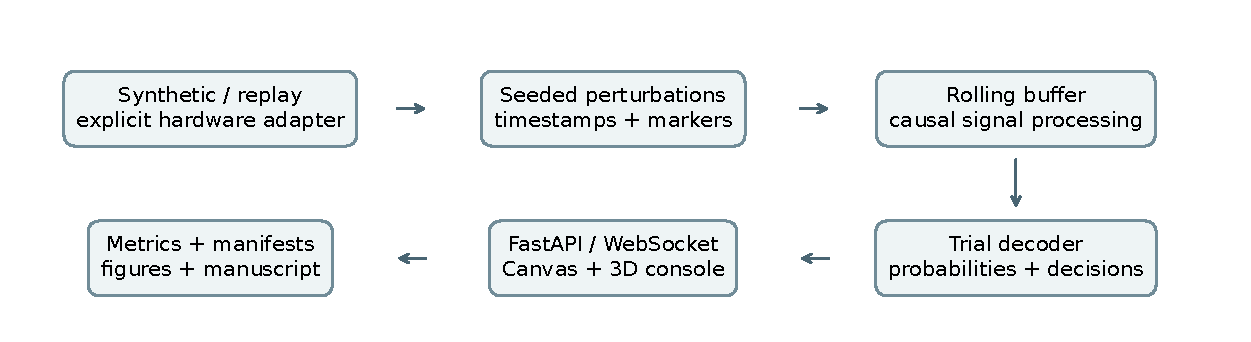
\includegraphics[width=\linewidth]{figures/architecture.pdf}
\caption{Software dataflow. Acquisition metadata and session-relative timestamps travel with signal chunks. Numerical outputs are logged before publication generation. The architecture diagram is conceptual, not an experimental measurement.}
\label{fig:architecture}
\end{figure}
The source contract provides connect, start, read, stop, and close operations. Metadata records the source category, sample rate, channel order, units, board identifier when applicable, and dataset, subject, and session when available. Signals are represented as channel-by-sample arrays in microvolts. Replay timestamps are session-relative sample times. Playback speed changes wall-clock delivery without changing source time. BrainFlow timestamps retain relative acquisition timing. They are checked for monotonicity rather than replaced by the time of a polling call.

Replay emits bounded chunks and carries start and end markers for every selected trial. Pause, resume, seek, looping, and speed controls are implemented. Loop offsets keep source timestamps increasing. A seek resets downstream buffers and suppresses incomplete-trial predictions. Accelerated replay uses the same read interface but omits pacing delays. The demonstration concatenates held-out task epochs, so it preserves task-trial boundaries but does not reproduce intervening rest periods or the complete original session chronology.

A bounded rolling buffer accepts ordered chunks, counts timestamp gaps, rejects late chunks, and extracts overlapping complete windows. Stateful causal filtering is available for continuous processing. The application displays raw traces and spectra. Its recorded decoding demonstration waits for a complete trial and applies the declared trial-local preprocessing used in evaluation. That is stream delivery followed by trial-end offline preprocessing, not a claim of sample-by-sample causal classification. A real hardware adapter is designed around BrainFlow acquisition, but physical-device connection requires explicit configuration and permission in the Python interface.

FastAPI exposes local REST control and a versioned WebSocket message envelope. One producer acquires and processes data independently of client drawing. Bounded client queues discard stale frames when a browser falls behind. Signal delivery targets a modest display cadence, spectra update less frequently, and trial predictions are independent of Canvas rendering. A temporal layer applies exponential smoothing, confidence gating, dwell time, and a refractory interval. Accuracy uses raw trial probabilities, without smoothing or future samples. The Three.js control object follows decoder decisions only in recorded mode. Synthetic mode uses a visibly identified deterministic control signal.

Session exports include source metadata, predictions, decisions, perturbations, timing, events, and configuration. Raw EEG is omitted by default. Default services bind to loopback, and the application has no analytics or EEG uploads. Saved models use numeric NPZ arrays or safetensors, JSON metadata, and weight checksums. Exact channel order and sampling frequency are checked before replay inference.

\section{Data and experimental protocol}
\begin{table}[t]
\centering\begin{tabular}{lrrrrr}
\toprule
Dataset & Subjects & Train & Test & Channels & Hz \\
\midrule
PhysionetMI & 5 & 150 & 75 & 3 & 160 \\
BNCI2014\_001 & 3 & 432 & 432 & 3 & 250 \\
\bottomrule
\end{tabular}

\caption{Included cohort and complete-trial counts, generated from the completed experiment manifest. Train and test counts are totals within each dataset. Both tasks are imagined left and right hand movement.}
\label{tab:cohort}
\end{table}
The PhysioNet EEG Motor Movement/Imagery Dataset \citep{physionet} is accessed with MNE's EEGBCI reader. Subjects 1 through 5 are included. Runs 4 and 8 provide training trials and run 12 supplies the held-out test run. These runs use hand imagery rather than executed movement. T1 and T2 task onsets are mapped to left and right hand classes. Baseline and non-hand imagery runs are not included. BNCI2014\_001, originally BCI Competition IV dataset 2a \citep{bnci}, supplies subjects 1 through 3. Its first session is used for training and its second session for testing. Only left and right hand trials are retained. These are within-subject cross-run and cross-session experiments, not cross-subject transfer.

C3, Cz, and C4 are selected in a fixed order on both datasets. Table~\ref{tab:cohort} reports the sampling rates and actual counts. Each epoch spans 0.5 to 3.5 seconds after the dataset task event, with the endpoint excluded. No resampling is needed. The adapter retains valid complete epochs, without a new amplitude-based rejection rule. The BNCI adapter uses the dataset's default artifact policy, so marked trials are not selectively removed for improved accuracy. No subject is excluded because of decoder performance.

A fourth-order Butterworth bandpass from 8 to 30 Hz is applied forward and backward within each trial after perturbation. Trial means are removed. No notch or additional reference is applied. Filtering within the complete trial has access to its future samples, but neither the training nor test filter accesses a different trial. This protocol must be distinguished from stateful causal filtering in continuous acquisition. The decoder receives \EpochSeconds{}-second windows and predicts once per complete test trial.

The frozen configuration specifies seed \SeedValue{} for splits, noise, model initialization, and bootstrap resampling. Models, normalization, CSP, and classifiers are fitted on training trials. EEGNet selects checkpoints using an inner stratified split from the training portion. Its inner scaling statistics are computed only from the inner training trials. No final test labels enter model fitting or adaptation. Automated checks require disjoint trial identifiers and preserve them in prediction artifacts. The design was frozen after a single-subject smoke test and before examining the full cohort outputs.

\section{Decoders and reference adaptation}
For a filtered trial $X\in\mathbb{R}^{C\times T}$, the bandpower baseline uses $\log(\epsilon+T^{-1}\sum_t X_{c,t}^2)$ for each channel. Features are standardized using training means and standard deviations. A logistic regression with fixed regularization produces binary probabilities. This is an interpretable pipeline-integrity reference rather than a detailed frequency-bank model.

CSP uses regularized class covariance estimates. A spatial filter solves the generalized variance-ratio problem
\begin{equation}
\Sigma_0 w = \lambda(\Sigma_0+\Sigma_1)w.
\end{equation}
MNE's implementation estimates covariance with oracle-approximating shrinkage and learns the spatial basis on training trials. At most four components are retained, limited by the available channels. In this experiment all three spatial components are used. Log projected mean-square features are standardized with training statistics and passed to shrinkage LDA. Weight arrays and classifier coefficients are stored without executable object serialization.

EEGNet uses Braindecode's temporal, depthwise spatial, and separable convolution implementation. Its configuration uses eight temporal filters, a depth multiplier of two, and dropout probability 0.25. The optimizer is Adam with learning rate 0.001 and batch size 16. A stratified 20\% training-only validation subset controls early stopping with patience eight. Training runs for at most \MaxEpochs{} epochs on one CPU thread. Validation curves, selected epoch, architecture settings, and safe checkpoints are retained in model metadata. This intentionally short laptop configuration is not an optimized deep-learning comparison.

The unlabeled adaptation strategy aligns per-channel expanding RMS to a fixed training reference. If $r_c$ is the training RMS and $\hat r_{c,k}$ is the RMS over centered test samples through trial $k$, the adapted signal is
\begin{equation}
 X'_{c,t}=\operatorname{clip}\left(\frac{r_c}{\max(\hat r_{c,k},\epsilon)},\frac14,4\right)(X_{c,t}-\bar X_c).
\end{equation}
Statistics include the current complete trial but no future trial. They reset for each subject, decoder, and shift condition. No test task label is accepted by this interface. The strategy can compensate gain changes but cannot recreate dropped-channel information, remove arbitrary additive noise, or guarantee improved classification. Correction clipping limits amplification of flat channels.

\section{Controlled distribution shift and metrics}
For each channel, $r_c^{\rm raw}$ is the centered broadband RMS measured only in training data. Gaussian perturbation is
\begin{equation}
\widetilde X_{c,t}=X_{c,t}+\alpha r_c^{\rm raw}N_{c,t},\qquad N_{c,t}\sim\mathcal N(0,1).
\end{equation}
The noise intensities are 0.5, 1, and 2. Perturbation precedes bandpass filtering, so these values describe broadband injected noise, not the final in-band signal-to-noise ratio. The same seed and chronological test order permit matched scenario comparisons across decoders.

Amplitude shift multiplies every channel by two. Drift adds a 0.2 Hz sinusoid with amplitude twice training raw RMS, evaluated on the concatenated trial-relative time axis. Fixed dropout masks C3, then C3 and C4, leaving channels present but zero-valued. The mixed condition combines noise intensity one with gain two. These settings provide interpretable stress tests, not realistic probability distributions of field artifacts. The software additionally implements line noise, channel-specific noise, random dropout, sample loss, interruptions, and timing jitter. Those transport-oriented cases are tested as engineering behavior, but no offline accuracy claims for them are included in this paper.

Accuracy, balanced accuracy, ROC AUC, F1, Brier score, and confusion matrices are stored per subject and condition. Balanced accuracy is the primary descriptive metric. Aggregation first computes each subject's score, then an unweighted dataset mean. Percentile confidence intervals use \BootstrapSamples{} subject-resampled bootstrap replicates and are descriptive in these very small cohorts. Adaptation contrasts use paired subject differences. We do not treat trials as independent participants, conduct formal hypothesis tests, or claim statistical superiority.

Inference timing is measured separately after warm-up with \LatencyCalls{} single-window calls using a monotonic high-resolution clock. The reported median and P95 are dataset medians of subject-model timing summaries. They exclude preprocessing, acquisition, WebSocket transport, and browser rendering. Separate software-processing profiles exercise real BrainFlow synthetic acquisition and accelerated held-out replay. They measure the source-read through frame-construction code path, not physical or end-to-end human control latency.

\section{Results}
\begin{table}[t]
\centering\begin{tabular}{lrrr}
\toprule
Decoder & BA (95\% CI) & Median (ms) & P95 (ms) \\
\midrule
Bandpower + LR & 60.9 [55.5, 66.2] & 0.008 & 0.009 \\
CSP + LDA & 55.9 [45.5, 70.0] & 0.010 & 0.011 \\
EEGNet & 44.6 [39.1, 49.1] & 0.158 & 0.188 \\
\bottomrule
\end{tabular}

\caption{PhysioNet held-out-run balanced accuracy (BA), expressed as a subject mean percentage with a descriptive subject-bootstrap 95\% interval. Inference timing summaries are medians across the included subject models, using a single complete trial per call. P95 denotes the median of per-model 95th percentiles.}
\label{tab:physio}
\end{table}
\begin{table}[t]
\centering\begin{tabular}{lrrr}
\toprule
Decoder & BA (95\% CI) & Median (ms) & P95 (ms) \\
\midrule
Bandpower + LR & 67.1 [52.8, 84.7] & 0.009 & 0.009 \\
CSP + LDA & 73.1 [53.5, 87.5] & 0.011 & 0.011 \\
EEGNet & 50.0 [47.9, 52.1] & 0.179 & 0.189 \\
\bottomrule
\end{tabular}

\caption{BNCI held-out-session balanced accuracy and inference timings, with the same aggregation and interval definitions as Table~\ref{tab:physio}. The cohort is exploratory and the interval does not establish decoder ranking.}
\label{tab:bnci}
\end{table}
Clean CSP plus LDA reaches mean balanced accuracy \PhysioCSPClean{}\% on PhysioNet and \BNCICSPClean{}\% on BNCI. The bandpower reference reaches \PhysioBandpowerClean{}\% and \BNCIBandpowerClean{}\%. EEGNet reaches \PhysioEEGNetClean{}\% and \BNCIEEGNetClean{}\% under the fixed short training schedule. Tables~\ref{tab:physio} and \ref{tab:bnci} give subject-level uncertainty and local inference costs. A decoder ranking would be premature given the limited training set, validation budget, and broad intervals.

\begin{figure}[t]
\centering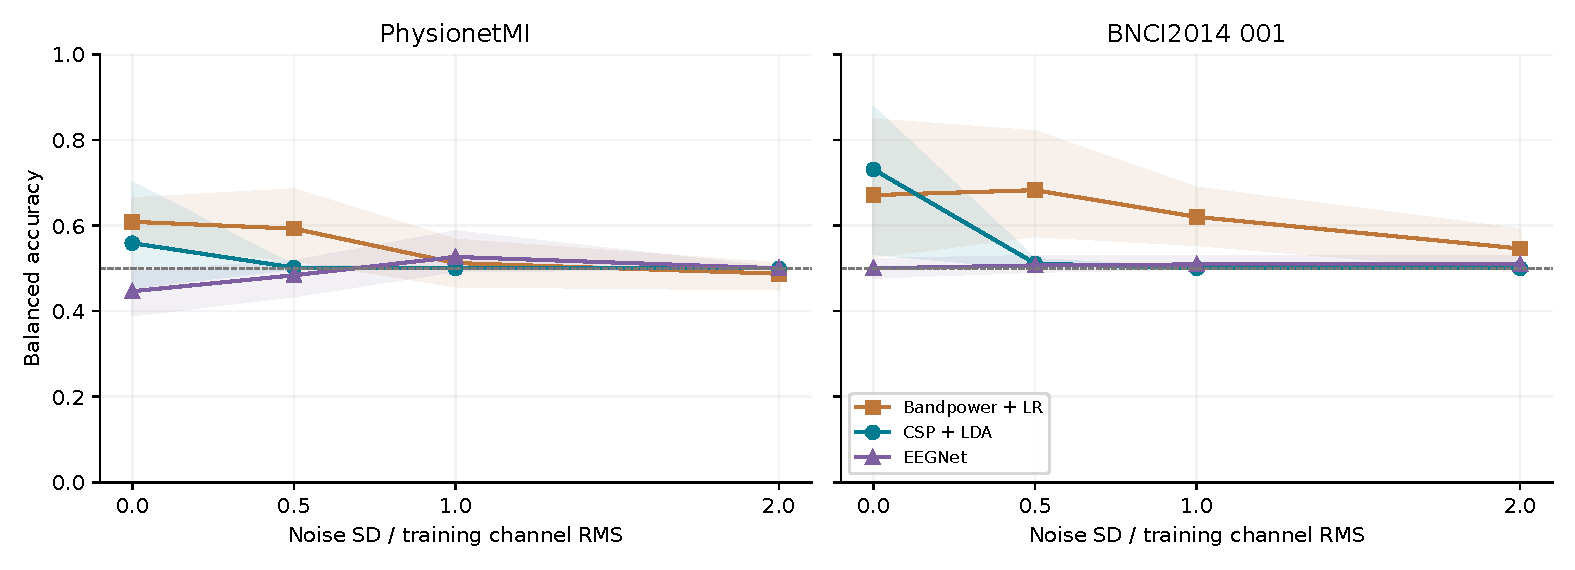
\includegraphics[width=\linewidth]{figures/noise.pdf}
\caption{Noise robustness on PhysioNet held-out runs and BNCI held-out sessions. Points are means of subject balanced accuracy. Shaded regions are descriptive 95\% subject-bootstrap intervals. Noise standard deviation is specified relative to training-only broadband channel RMS and applied before filtering. Dashed lines indicate binary balanced-accuracy chance level. No adaptation is used.}
\label{fig:noise}
\end{figure}
At noise intensity two, CSP plus LDA means are \PhysioCSPNoise{}\% and \BNCICSPNoise{}\%. Figure~\ref{fig:noise} reports the complete severity curves rather than assuming monotonic degradation for every model. Perturbations can interact with a model's feature normalization and with existing dataset shift. A stress condition can occasionally change a small-cohort mean favorably, which is not evidence that noise improves decoding generally.

\begin{figure}[t]
\centering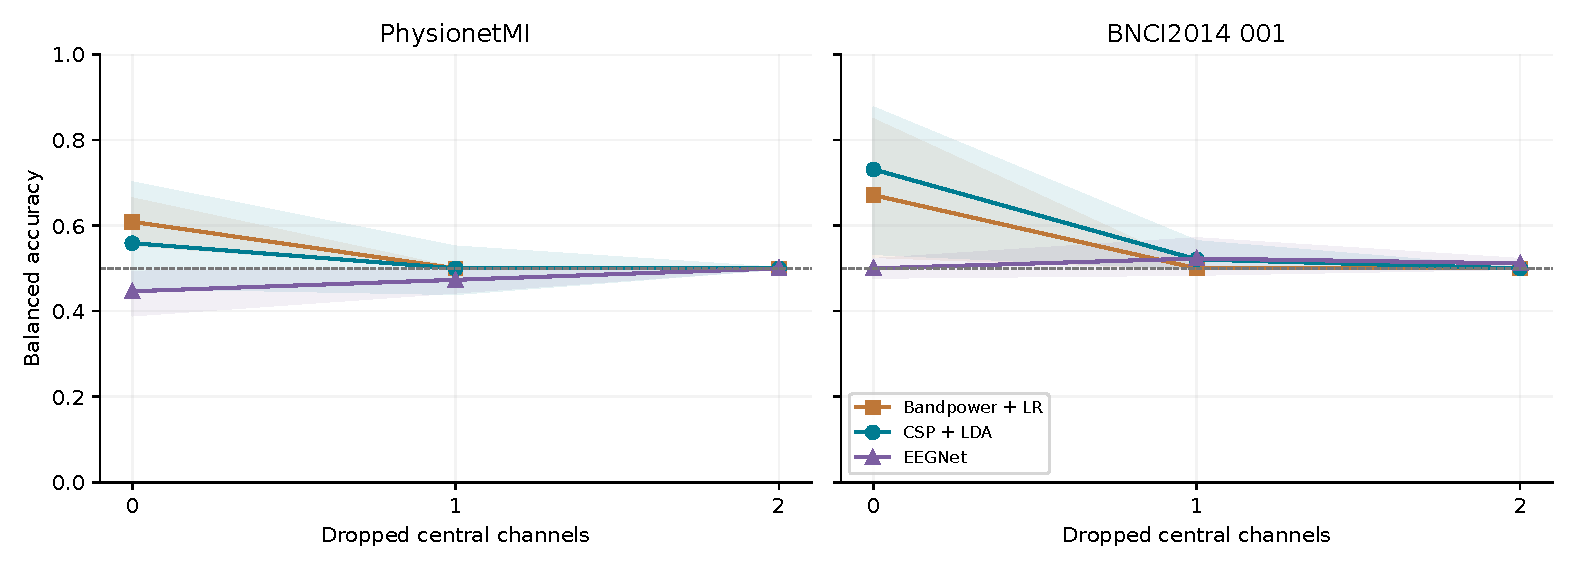
\includegraphics[width=\linewidth]{figures/dropout.pdf}
\caption{Fixed central-channel loss with no adaptation. Zero loss is clean, one removes C3, and two remove C3 and C4. The remaining channel for the largest loss is Cz. Curves show subject mean balanced accuracy with descriptive 95\% subject-bootstrap intervals on the same held-out trials as the noise experiment.}
\label{fig:dropout}
\end{figure}
With C3 and C4 lost, CSP plus LDA reaches \PhysioCSPDropout{}\% on PhysioNet and \BNCICSPDropout{}\% on BNCI. Figure~\ref{fig:dropout} characterizes a restricted electrode-loss scenario. It does not estimate robustness to arbitrary montages or optimize a reduced sensor layout.

\begin{table}[t]
\centering\begin{tabular}{llrr}
\toprule
Dataset & Decoder & Shifted BA & RMS BA \\
\midrule
PhysionetMI & Bandpower + LR & 50.5 & 51.1 \\
PhysionetMI & CSP + LDA & 49.1 & 51.8 \\
PhysionetMI & EEGNet & 50.4 & 45.9 \\
BNCI2014\_001 & Bandpower + LR & 63.9 & 68.8 \\
BNCI2014\_001 & CSP + LDA & 62.3 & 73.1 \\
BNCI2014\_001 & EEGNet & 50.5 & 51.2 \\
\bottomrule
\end{tabular}

\caption{Amplitude-shift comparison. Values are subject mean balanced accuracy percentages. Shifted BA uses gain two without adaptation. RMS BA uses gain two with expanding unlabeled channel-RMS alignment. Paired subject-bootstrap differences for all shifts are stored in the statistics artifact.}
\label{tab:adaptation}
\end{table}
\begin{figure}[t]
\centering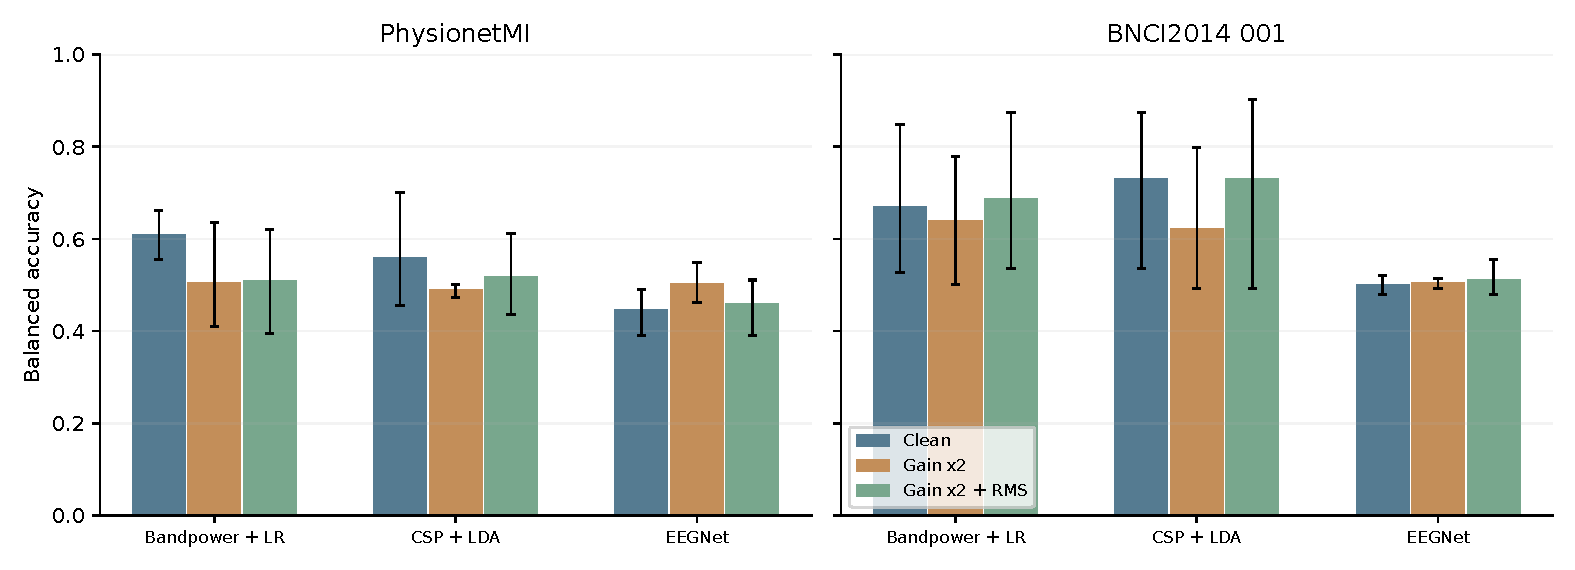
\includegraphics[width=\linewidth]{figures/adaptation.pdf}
\caption{Clean, gain-two, and gain-two with unlabeled RMS alignment. Bars show dataset subject mean balanced accuracy. Error bars are descriptive 95\% subject-bootstrap intervals. Statistics include the current complete trial and preceding trials, with no task labels or future trials.}
\label{fig:adaptation}
\end{figure}
For the gain-two condition, CSP plus LDA changes from \PhysioCSPAmplitude{}\% to \PhysioCSPAdapted{}\% on PhysioNet and from \BNCICSPAmplitude{}\% to \BNCICSPAdapted{}\% on BNCI under RMS alignment. These are measured changes, not a universal recovery guarantee. Table~\ref{tab:adaptation} and Figure~\ref{fig:adaptation} show all three decoder baselines. Full per-subject metrics and paired descriptive intervals are retained for every condition.

\begin{table}[t]
\centering\begin{tabular}{lrrrr}
\toprule
Mode & Frames & Median (ms) & P95 (ms) & Predictions \\
\midrule
Synthetic & 120 & 0.798 & 1.286 & 0 \\
Replay & 500 & 0.092 & 0.295 & 16 \\
\bottomrule
\end{tabular}

\caption{Local software-processing profile. Synthetic mode uses actual BrainFlow synthetic acquisition. Replay is accelerated held-out PhysioNet trial delivery through the CSP decoder. Times cover source read through frame construction and exclude network transport and browser rendering. Frames are the measured software-processing calls, not independent trials.}
\label{tab:streaming}
\end{table}
The local machine is an arm64 macOS host running Python 3.12, with software versions recorded in the run manifest. Synthetic processing has median \SyntheticPipelineMedian{} ms and P95 \SyntheticPipelinePninetyfive{} ms. Accelerated replay has median \ReplayPipelineMedian{} ms and P95 \ReplayPipelinePninetyfive{} ms across \ReplayFrames{} frames, producing \ReplayPredictions{} complete-trial predictions. Synthetic timestamps produce \SyntheticGaps{} nominal missing-sample counts under the buffer's sample-interval rounding rule. Replay produces \ReplayGaps{}. These counters are timing diagnostics, not proof of physical packet loss. Replay's median mainly reflects non-inference chunks, so it is not a decoder latency estimate.

\section{Reproducibility and limitations}
The frozen YAML design is linked by hash to raw probability arrays, subject metrics, aggregated intervals, generated tables, generated prose macros, and numerical figures. A provenance checker recomputes classification metrics from probability artifacts, checks trial separation, checks model metadata hashes, and rejects stale tables or missing files. A separate streaming profile stores its raw duration samples. Publication commands compile the manuscript, scan source and extracted PDF punctuation, inspect missing references, and compile the arXiv bundle from its own directory. Software version \SoftwareVersion{} is a pre-release research implementation.

This evaluation is limited to the included subjects and three central electrodes. It does not establish cross-subject generalization, population-level statistical superiority, online user performance, or clinical effectiveness. Short EEGNet training and limited validation make architectural conclusions inappropriate. The small subject-bootstrap samples cannot characterize the tails of population uncertainty reliably.

Replay supplies recorded tasks, not the current user's intention. Concatenating task epochs removes real inter-trial rest periods. Trial-local zero-phase preprocessing differs from the causal continuous filter. Pacing and browser scheduling are software behaviors and cannot replace measurement of acquisition-device jitter. The tested profile excludes browser drawing and transport latency, and the hardware adapter remains unvalidated on a physical board.

RMS alignment assumes that part of the shift can be represented as channel amplitude changes. It can normalize informative amplitude differences away, respond poorly to persistent additive artifacts, and cannot reconstruct missing channels. Transport perturbations and continuous running decisions remain engineering tests rather than additional human accuracy experiments. Dataset licenses are independent of the software license, and recordings and modified EEG are not redistributed with the repository.

\section{Conclusion}
\project{} provides a local hardware-free path from timestamped acquisition and held-out EEG replay to interactive software and reproducible robustness reports. The completed experiments show how established decoders respond to fixed noise, channel loss, and gain scenarios under explicitly declared preprocessing. Conservative unlabeled alignment can be studied within the same artifact chain without assuming it always helps. Future work should validate the source contract on physical acquisition, evaluate larger cohorts and electrode sets, and compare causal continuous decoding with the trial-end protocol used here.

\section*{AI assistance disclosure}
OpenAI Codex generated software, executed the reported computational experiments and automated checks, and drafted manuscript text under the author's instructions. AI assistance also supported literature searches, figures, and publication packaging. AI systems are not listed as authors. These computational checks do not replace independent scientific review.

\begingroup
\footnotesize
\setlength{\bibsep}{2pt}
\bibliographystyle{abbrvnat}
\bibliography{refs}
\endgroup
\end{document}
